In situations where multiple agents are required to make decisions, it is necessary to elect a leader among the agents to facilitate the decision-making process. The elected leader will assume responsibility for generating a map and for transmitting relevant data about the swarm to other relevant services (e.g. the backend system). The primary algorithm utilized for leader election is depicted in Figure \ref{fig:election_logic}. 

\begin{figure}[H]
    \centering
    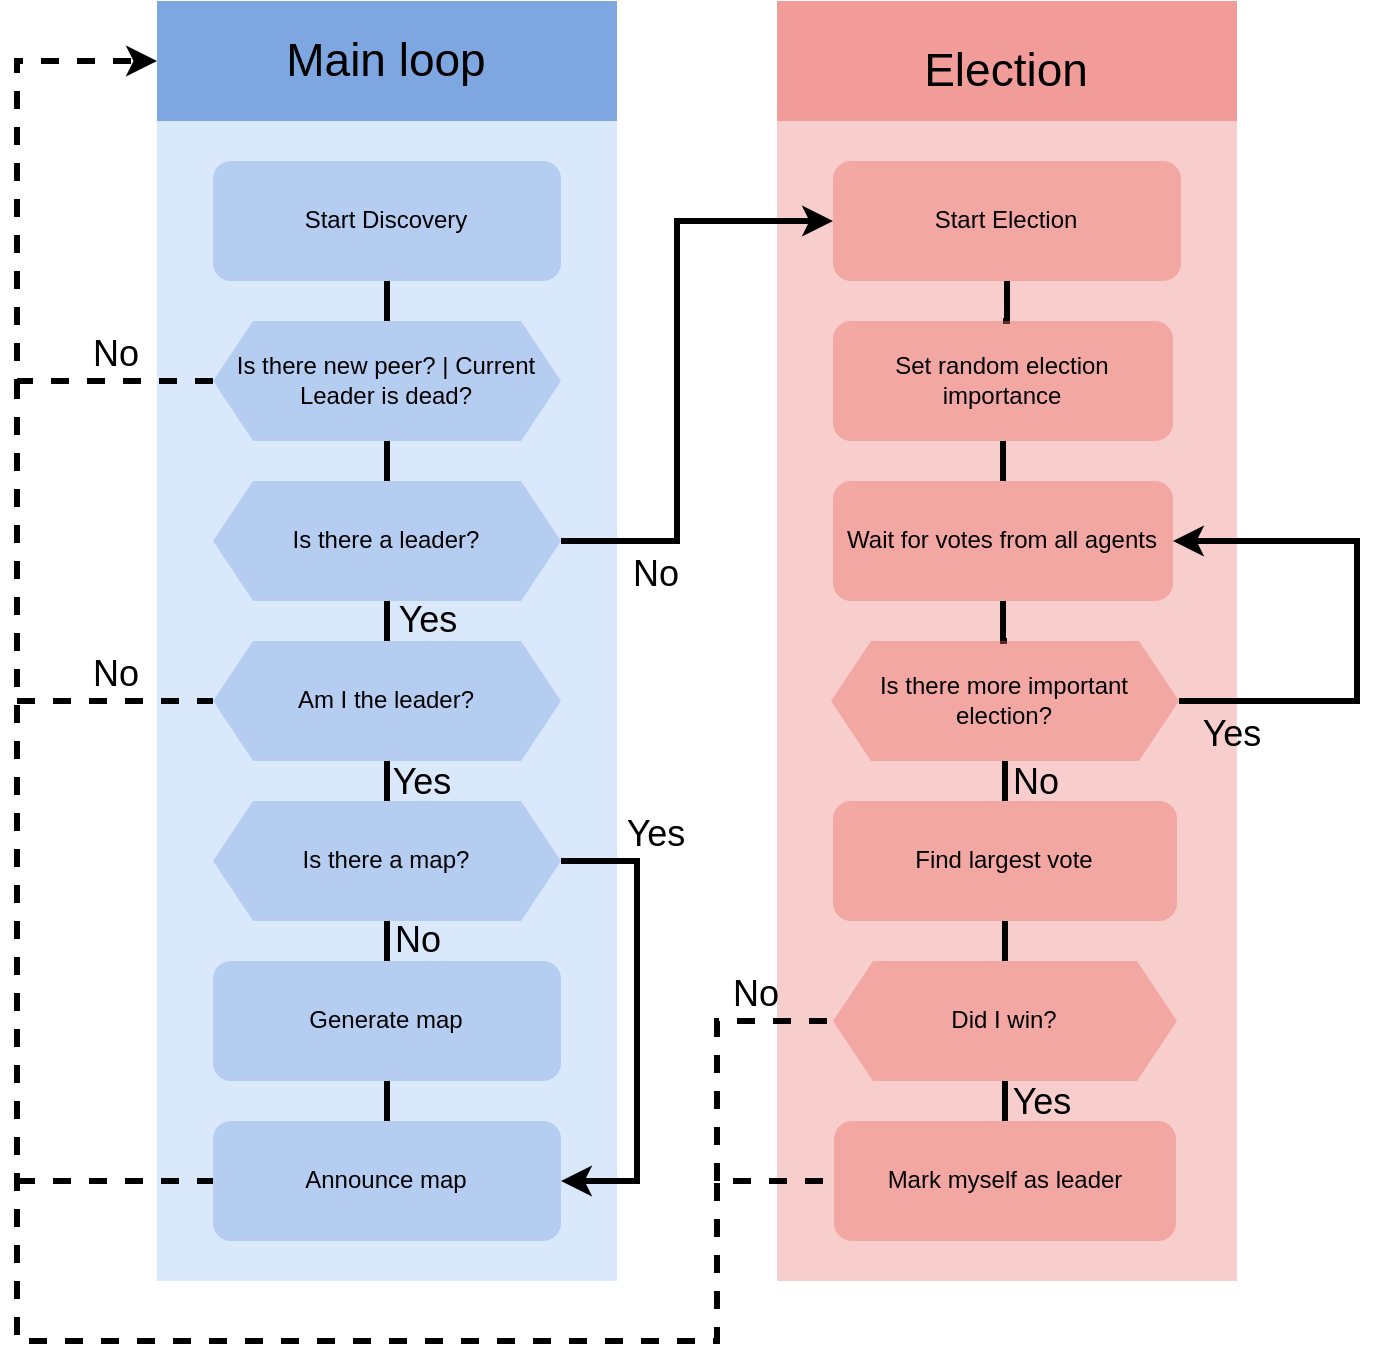
\includegraphics[width=0.8\textwidth]{pictures/election_logic.png}
    \caption{Election logic}
    \label{fig:election_logic}
\end{figure}

The leader election algorithm described is triggered under specific conditions, namely the discovery of a new peer or the failure of the current leader to maintain connectivity. Additionally, it is a requirement that there is no already elected leader. Upon the occurrence of these conditions, an agent initiates the election process by broadcasting a message to other agents, including a randomly generated number that serves as a signal of the importance of the election. Multiple elections can be concurrently initiated by multiple agents.

After initiating an election, the agent enters a waiting state during which it receives votes from other agents. However, if the agent receives a message indicating the initiation of a more important election (f.e. one with a higher randomly generated number), it will discontinue its current election and participate in the more important one. Once all votes are received, the agent with the highest vote is declared the leader and announced as such to the other agents, who subsequently accept it as the leader. To avoid conflicts, the randomly generated numbers used for both voting and signaling election importance should be set to large values.